\chapter{Digital pathology}
\label{chap:backdp}

\begin{overview}{Overview}
  The goal of this chapter is to provide digital pathology background  and keys to understand our contributions. We will focus our attention on topics relevant to this thesis. 
  
  Section \ref{sec:backdp:whatisdp} introduces and defines medical terms such as \textit{pathology}, defines \acrfirstit{dp} and introduces the notion of \acrfirstit{wsi}. Section \ref{sec:backdp:wsi} presents the journey of a sample from the body to the \acrshort{wsi}, introducing the different sources of variability introduced by the whole conversion process. 
\end{overview}

% analogintelligence.com image dp illustration

\section{What is digital pathology?}
\label{sec:backdp:whatisdp}

Nowadays, medicine and healthcare rely heavily on analysis of human body samples to study and diagnose diseases. The branch of medicine focusing on this analysis is called \textit{pathology} which includes histology-based pathology (\aka histopathology) and cytology-based pathology (\aka cytopathology). Both of these sub-branches involve the study of microscope glass slides containing samples (see Figure \ref{fig:backdp:glassslides}). In the case of histology, these samples are tissue sections cut from a bodily specimen. Cytology, on the other hand, is concerned with samples of free cells or tissue fragments which can be extracted by different techniques. 

\begin{figure}
  \centering
  \subfloat[Glass slide]{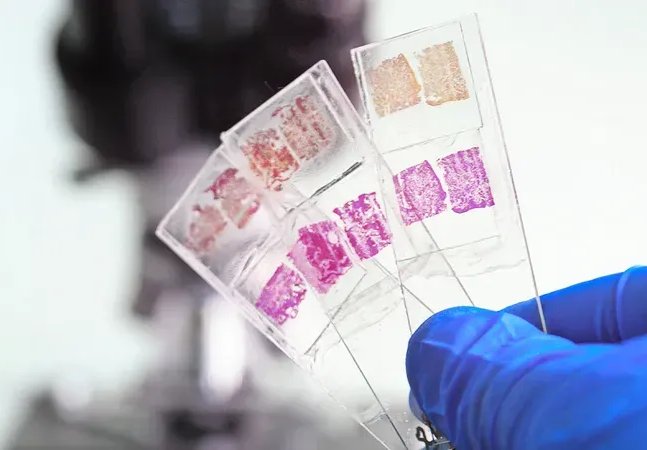
\includegraphics[scale=0.35]{backdp/microscope-slide.png}}\quad
  \subfloat[Whole-slide image]{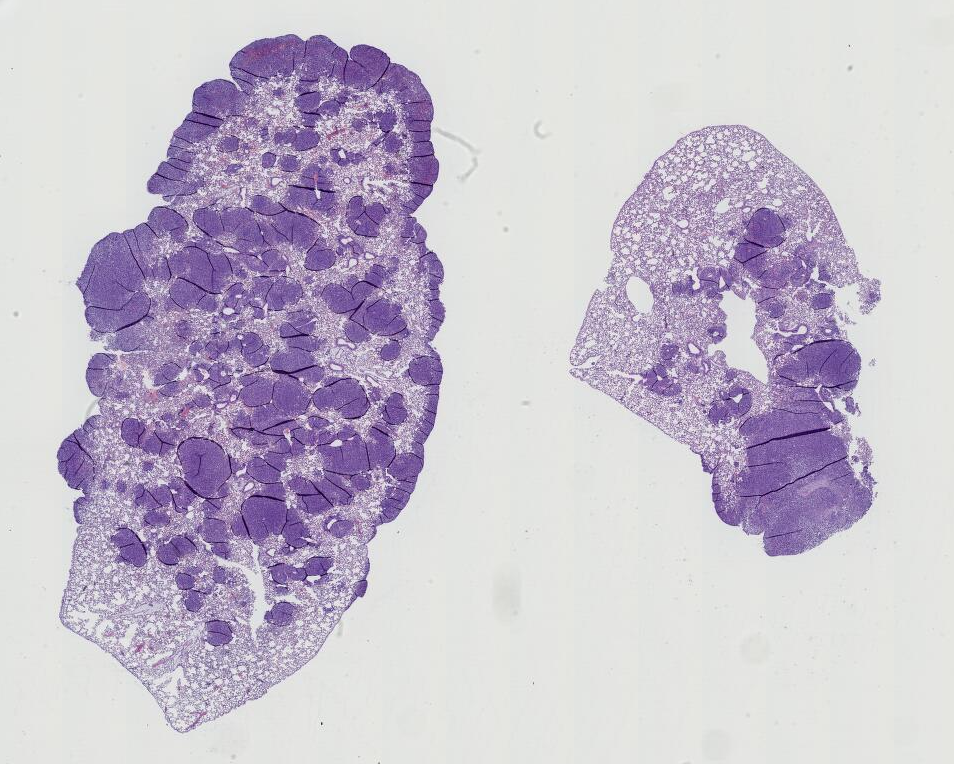
\includegraphics[scale=0.22]{backdp/wsi.png}}
  \caption{Microscope slides with tissue samples (images from \parencite{img:glassslides} and \TODO{reference demo cytomine}).}
  \label{fig:backdp:glassslides}
\end{figure}

The trend of digitalization affecting our societies also impacts pathology as, using dedicated scanners, these glass slides can now be digitized into large image files called \acrfirstit{wsi}. In this context, \acrfirstit{dp} can be defined as ``\textit{the acquisition, management, sharing and interpretation of pathology information — including slides and data — in a digital environment}'' \parencite{doolan2019whatisdp}. Working with \acrshort{wsi} instead of physical slides has several advantages and drawbacks (see Table 1 in \parencite{jahn2020digital} for a thorough list). Aside from easier sharing and storing of slides, digitization also opens the way for automated analysis sofware to extract relevant information for pathologists. Such software have the potential to relieve pathologists from easy but time-consuming tasks allowing them to focus on challenging cases and research therefore reducing healthcare cost and improving quality. According to the 2020 report on cancer from \acrfirstit{who} \parencite{world2020report}, the ratio of pathologist per inhabitant is approximately 1 per 15000 in high income countries whereas it dramatically drops to 1 per 1 million in some African countries (sometimes less in other low income countries). AI-assisted pathology therefore holds even greater promises for coverage and quality of healthcare in these countries where pathologists are rare.  

Interestingly, although digitization technologies are quite mature, the adoption of \acrlong{dp} in healthcare facilities is not automatic. Many still heavily rely on glass slides for day-to-day operations. Indeed, the transformation requires significant investments (both in time and money) and careful planning to carry it out successfully which is not always comptabile with the workload of pathology services. Sometimes, experienced pathologists might also be reluctant to change and lack confidence in modern tools for slide visualization and analysis. 

Whereas automated processing of \acrshort{wsi} is possible, it remains quite a challenge. Whole-slide images typically contain several gigapixels and cannot be processed with classical computer vision tools without adjustements. The conversion from a body sample to a \acrshort{wsi} is a noisy process (see Section \ref{sec:backdp:wsi}) introducing sources of variability in the resulting image that might hamper the algorithms ability to achieve efficiently the task they were designed for.

\section{Whole-slide images: a journey from the body to the computer}
\label{sec:backdp:wsi}

Turning a body sample into whole-slide images is a long and complex multi-step process typically involving the work of several highly-specialized technicians. Some steps can nowadays be automated but the chain remains mostly manual. In this section, we describe the different steps and link them with possible sources of variability in the resulting \acrshort{wsi}. An alternate presentation of the process with illustrations can be found in \parencite{mccann2014automated}. 

\subsection{Collecting samples, fixing and cutting}

Whereas we focus mostly on histo- and cyto-pathology in this thesis, a pathology service typically deals with more than these two modalities. The samples they receive for analysis range from small, commonly referred to as \textit{biopsies}, to very large (whole organ or body). Whole bodies are usually destined for autopsies which might themselves generate biopsies. Smaller samples (organs, biopsies) must be fixated before going through the next steps \parencite{rolls2012process}. The goal of fixation is to put a stop to the natural decay of the sample and increase its structural stability. There exists several approaches to achieve this. For instance, a common approach consists in immersing the sample in a formaldehyde bath (\ie the fixative solution). Bad fixation can result in decaying tissue and structural degradation which can make analysis more difficult or impossible (see Figure \ref{fig:backdp:fixation}). Duration of fixation vary as a function of the size of the sample. It lasts few hours for very small samples but can reach 24 hours for large ones. 

When the sample has been fixated\TODO{cytology: also cut ?)}, it must be placed into a standardized container called a \textit{cassette} (see Figure \ref{fig:backdp:cassette}). If it is too large for the cassette, one must extract a smaller volume by cut. The cutting tool can also introduce artifacts.  

\begin{figure}
  \centering
  \subfloat[This is an example of well-fixed tissue showing good nuclear and cytoplasmic morphology with minimal shrinkage showing clearly defined basement membranes and cell margins.]{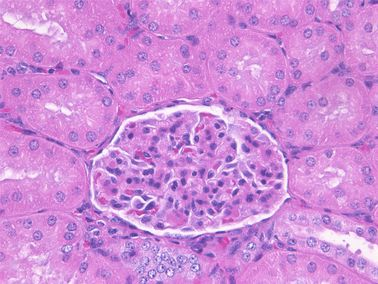
\includegraphics[scale=1.0]{backdp/fixationgood.png}\label{fig:backdp:goodfixation}}\quad
  
  \subfloat[This is an example of poorly-fixed tissue showing inferior nuclear and cytoplasmic morphology with excessive shrinkage and poorly defined cell margins.]{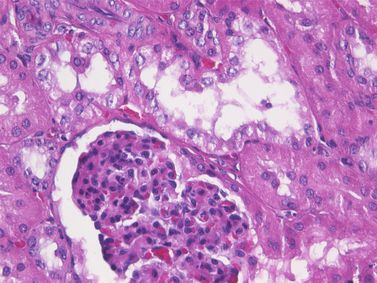
\includegraphics[scale=1.0]{backdp/fixationbad.jpg}\label{fig:backdp:badfixation}}
    
  \caption{Examples of good and bad fixations (images and sub-captions from \parencite{rolls2012process}).}
  \label{fig:backdp:fixation}
\end{figure}

\begin{figure}
  \centering
  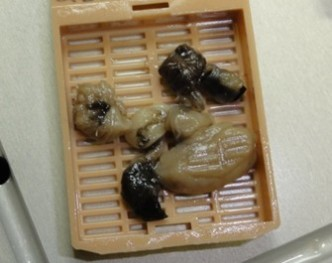
\includegraphics[scale=0.85]{backdp/cassette.jpg}
  \caption{A standard tissue cassette (image from \parencite{stidworthy2011getting})}
  \label{fig:backdp:cassette}
\end{figure}

\subsection{Biopsy and smearing}
\subsection{Staining}
\subsection{Scanners}

\section{Professions and typical tasks}
\label{sec:backdp:professionandtasks}

\section{Machine learning}
\label{sec:backdp:ml}

\subsection{Data leakage}
\label{ssec:backdp:dataleakage}

\subsection{Data scarcity}
\label{ssec:backdp:datascarcity}
% and imperfect annotations

\subsection{Transfer learning}
\label{ssec:backdp:tl}

\parencite{van2019strategies}

\section{Visualization and analysis tools}

\subsection{Cytomine}

\subsection{Others}

\section{Digital pathology datasets}
\label{sec:backdp:dataset}


% origin, acknowledgements, subject, organ, staining, statistics


\subsection{Thyroid nodule fine-needle aspiration biopsy}



\subsection{Publicly available}